\documentclass[11pt]{article}

\usepackage[a4paper,margin=27mm]{geometry}
\usepackage[T1]{fontenc}
\usepackage[utf8]{inputenc}
% Times-like text and math as in the preceding studies' manuscripts when newtx is installed; otherwise mathptmx.
\usepackage{amsmath}
\usepackage{amsthm}
\IfFileExists{newtxtext.sty}{\usepackage{newtxtext}\usepackage{newtxmath}}{\usepackage{mathptmx}}
\usepackage{microtype}
\usepackage{booktabs}
\usepackage{tabularx}
\usepackage{graphicx}
\usepackage{float}
\usepackage{caption}
\usepackage{enumitem}
\usepackage{xcolor}
\usepackage{seqsplit}
\usepackage{tikz}
\usetikzlibrary{positioning,arrows.meta}
\usepackage[hidelinks]{hyperref}

\microtypesetup{protrusion=false}
\setlength{\emergencystretch}{3em}
\captionsetup{font=small,labelfont=bf}
\renewcommand{\topfraction}{0.9}
\renewcommand{\textfraction}{0.07}
\renewcommand{\floatpagefraction}{0.85}
\setlist[itemize]{leftmargin=*,topsep=3pt,itemsep=1pt}
\setlist[enumerate]{leftmargin=*,topsep=3pt,itemsep=2pt}

\theoremstyle{plain}
\newtheorem{proposition}{Proposition}
\newtheorem{observation}{Observation}
\theoremstyle{definition}
\newtheorem{definition}{Definition}

\newcommand{\argine}{\textsc{Argine}}
\newcommand{\code}[1]{\texttt{\seqsplit{#1}}}
\newcommand{\hsh}[1]{\texttt{\seqsplit{#1}}}
\newcommand{\gate}[1]{{\itshape\fontsize{6}{7}\selectfont #1}}
\newcommand{\nuex}{\textsc{nue-x}}
\newcommand{\bel}{B_{\star}}

\title{\textbf{Causal State Is Not Enough:\\
Prospective Evidence That Tested Causal Eviction Policies Recover\\
Too Little Clairvoyant Headroom in Expert Retention}}
\author{sennape}
\date{November 2026}

\begin{document}
\maketitle

\begin{abstract}
Serving a Mixture-of-Experts model from a fixed memory budget requires an online rule for which expert weights to keep resident. A clairvoyant eviction rule (Belady) bounds what any such rule could save, and earlier studies in this series found that this clairvoyant headroom is large, that expert routing contains causal predictive structure, and that prediction-led retention nevertheless produced no net runtime benefit. We ask whether the remaining obstacle is the causal state available to an online eviction policy: how much of the clairvoyant miss-byte headroom can causal policies recover, and can a rich causal decision rule be distilled into a deployable rule of a few integer comparisons? We replay frozen routing traces of Qwen3-30B-A3B-Q4\_K\_M offline at a 1.5~GiB expert budget. A gradient-boosted regression-tree policy and a depth-3 decision tree are fitted on four development traces, scored once on twelve validation traces, and scored once on four prospective held-out traces; the headroom captured is the pooled fraction of baseline miss bytes that a policy recovers relative to the clairvoyant reference. Belady removes $41.85\%$ of the baseline's miss bytes on the held-out traces. A frozen rule required at least $25\%$ capture on both splits. Two hand-built causal comparators capture at most $7.42\%$ (validation) and $9.37\%$ (held-out); the rich learned policy captures $15.45\%$ and $19.11\%$, about twice as much, but below the requirement; and the distilled cheap policy captures $-36.04\%$ and $-29.96\%$, that is, it incurs more miss bytes than the baseline on every one of the sixteen traces. No tested policy meets the requirement, so within the frozen feature vocabulary, model families and regime the causal state is insufficient. The result does not show that causal or learned eviction is impossible in general, and the clairvoyant reference is not a deployable target.
\end{abstract}

%=====================================================================
\section{Introduction}
\label{sec:intro}

Mixture-of-experts (MoE) models activate a small subset of experts per token~\cite{shazeer2017sparsely,fedus2022switch}. When the expert weights do not fit in fast memory, inference systems keep a resident subset and load the rest on demand; a substantial body of systems work exploits routing behaviour through caching, offloading, scheduling or prediction~\cite{eliseev2023offloading,xue2025moeinfinity,kamahori2025fiddler,promoe2025,layerscope2025,expertflow2026}. In such a system the retention policy decides which resident expert to evict when a missed expert must be loaded, and its quality can be measured directly as the number of bytes that must be loaded again.

The series of studies to which this paper belongs has measured how much a retention policy could matter and why it has not yet paid off. A first study~\cite{argine2paper} found that, for one model and runtime, a clairvoyant Belady-style comparator~\cite{belady1966replacement} incurs far fewer miss bytes than a causal baseline, that expert routing carries causal predictive structure, and that a predictor-driven policy reduced miss bytes in offline replay but did not improve real decode throughput. A second study~\cite{argine3paper} then prospectively decomposed that outcome. It found that the best tested causal next-use predictive eviction policy captured only $8.79\%$ of the clairvoyant miss-byte headroom on its canonical stream and that the corrected predictive policy lost $15.83$~ms/token in a paired runtime experiment, while leaving open how much of the headroom is causally recoverable and whether a policy distilled from the clairvoyant optimum could do better.

The present study isolates that open question from runtime cost. It asks whether the obstacle to prediction-led expert retention is the \emph{causal state} on which an online eviction policy must decide, rather than the cost of computing the decision. Concretely: \emph{how much of the clairvoyant eviction optimum can causal policies recover, and can the recovery be preserved when a rich causal decision rule is compressed into a cheap, deployable one?} The question is answered offline, with exact integer accounting and zero charge for policy computation, so that any shortfall is a shortfall of information or of model class and not of overhead.

The answer we report is negative within the tested regime. Two hand-built causal comparators recover a small share of the headroom. A richer gradient-boosted policy over sixteen causal features recovers about twice as much, but still well below a frozen sufficiency level of $25\%$ on both validation and held-out data. A decision tree of depth at most three, trained to imitate the clairvoyant teacher and evaluated under its own cache state, performs worse than the baseline on every trace. Section~\ref{sec:claims} states precisely what these facts do and do not establish. Figure~\ref{fig:design} shows the design.

\begin{figure}[t]
\centering
% Figure 1: design of the study (reader-facing names; each box lists its role or frozen gate).
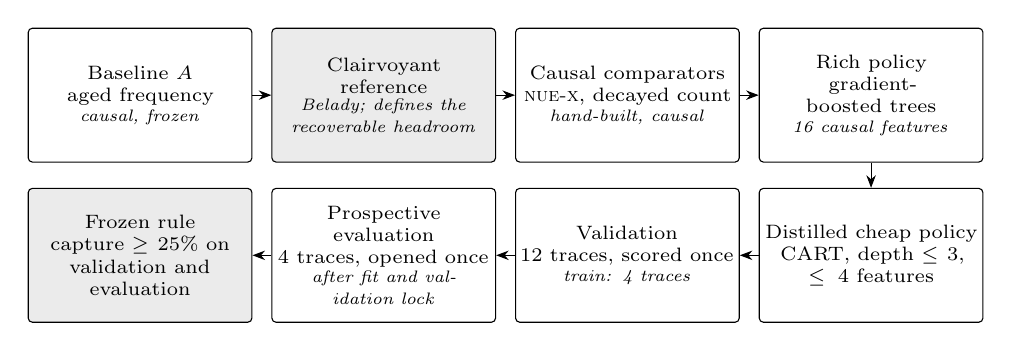
\begin{tikzpicture}[
  node distance=3.2mm and 2.4mm,
  box/.style={draw, rounded corners=1.5pt, align=center, font=\scriptsize, text width=27mm, minimum height=17mm, inner sep=2pt},
  ref/.style={box, fill=black!8},
  arr/.style={-{Stealth[length=1.6mm]}, thin}]
\node[box] (a) {Baseline $A$\\aged frequency\\[-1pt]\gate{causal, frozen}};
\node[ref, right=of a] (b) {Clairvoyant\\reference\\[-1pt]\gate{Belady; defines the\\recoverable headroom}};
\node[box, right=of b] (c) {Causal comparators\\\nuex, decayed count\\[-1pt]\gate{hand-built, causal}};
\node[box, right=of c] (d) {Rich policy\\gradient-boosted trees\\[-1pt]\gate{16 causal features}};
\node[box, below=of d] (e) {Distilled cheap policy\\CART, depth $\le 3$,\\$\le 4$ features};
\node[box, left=of e] (f) {Validation\\12 traces, scored once\\[-1pt]\gate{train: 4 traces}};
\node[box, left=of f] (g) {Prospective evaluation\\4 traces, opened once\\[-1pt]\gate{after fit and validation lock}};
\node[ref, left=of g] (h) {Frozen rule\\capture $\ge 25\%$ on\\validation and evaluation};
\draw[arr] (a) -- (b); \draw[arr] (b) -- (c); \draw[arr] (c) -- (d); \draw[arr] (d) -- (e);
\draw[arr] (e) -- (f); \draw[arr] (f) -- (g); \draw[arr] (g) -- (h);
\end{tikzpicture}

\caption{Design of the study, read right to left from the baseline. Gray boxes are references: the baseline $A$ and the clairvoyant reference define the recoverable headroom, and the frozen rule defines sufficiency. Policies are fitted on a training set only, scored once on a validation cohort, and scored once on a prospective held-out evaluation that was sealed until the fit and the validation scores were locked.}
\label{fig:design}
\end{figure}

%=====================================================================
\section{Background and Motivation}
\label{sec:background}

\subsection{Memory-Constrained Mixture-of-Experts Inference}
\label{sec:bg-moe}
The studied system serves Qwen3-30B-A3B-Q4\_K\_M~\cite{qwen3technicalreport} through a modified llama.cpp runtime~\cite{gerganov2023llamacpp}. The model has 48 MoE layers with 128 experts each and top-8 routing; experts have two byte sizes. An expert store keeps a byte-budgeted resident set of (layer, expert) objects; a request for a non-resident expert is a miss and the expert is loaded on demand (demand admission), evicting residents until the budget holds. The quantity of interest is the number of \emph{miss bytes}: the total size of experts that must be loaded because they were not resident.

\subsection{Expert Retention and Clairvoyant Headroom}
\label{sec:bg-headroom}
A retention policy chooses victims. Belady's rule evicts the resident whose next use lies farthest in the future~\cite{belady1966replacement}; it requires knowledge of the future and is therefore a reference and not a deployable policy. For multi-key events and two expert sizes it is not proven optimal, so the headroom it defines is a comparator-relative margin and not a proven bound on what any policy could achieve. We nevertheless use it as the denominator of every comparison, as the preceding studies did.

\subsection{Predictive Structure Without Runtime Value}
\label{sec:bg-pred}
The first study~\cite{argine2paper} established that routing has layer-local and transition structure that a strictly causal predictor can exploit on held-out data, and that a predictor-driven retention policy lowers miss bytes in offline replay. The second~\cite{argine3paper} tested the conversion of that information into runtime value under frozen economic criteria and found that, in its regime, it does not convert: the real-runtime net effect was a loss, and offline counterfactuals showed that the best tested causal next-use policy recovered a small share of the clairvoyant headroom even with zero policy-computation cost.

\subsection{The Remaining Causal-State Question}
\label{sec:bg-question}
That result left the representation question open. A policy that decides only from what has been observed (its causal state) might simply lack the information the clairvoyant rule uses, or the available information might be sufficient but hard to exploit with a hand-built rule. Learning a decision rule from clairvoyant supervision is an established idea in cache replacement: Hawkeye reconstructs Belady's decisions on past accesses to train a predictor~\cite{hawkeye2016}, Glider uses an offline-trained deep model to design a compact online predictor~\cite{glider2019}, and Parrot imitates Belady's policy conditioned on past accesses~\cite{parrot2020}. For expert caches, FlashMoE trains a small network on Belady-derived labels~\cite{flashmoe2026}, Bacon et al.\ compare history-based and learned causal eviction with a farthest-future reference in an offloading setting~\cite{bacon2026fewer}, and Zhang cautions that the offline-optimal gap can overstate what causal methods recover and that replay semantics and oracle definitions change conclusions~\cite{zhang2026reproducible}. None of these settings is the regime studied here (different models, hardware, workloads, byte budgets and accounting), and no novelty is claimed for the use of an oracle teacher or of recency, frequency and decayed-count features. The contribution is a prospectively frozen test of a specific, bounded question in one regime.

%=====================================================================
\section{Research Question and Hypotheses}
\label{sec:question}

\paragraph{Question.} Can a compact deployable eviction rule, distilled offline from clairvoyant next-use supervision but evaluated causally under its own cache state, recover enough of the clairvoyant miss-byte headroom to justify any later runtime implementation?

\paragraph{Preregistered hypotheses.} Four conditions were frozen before any validation or held-out statistic was read (Section~\ref{sec:rule}). (H1) \emph{Operational viability}: the distilled cheap policy captures at least $25\%$ of the headroom on validation and on held-out data. (H2) \emph{Incremental value}: on held-out data it exceeds the best hand-built causal comparator by at least three percentage points. (H3) \emph{Workload consistency}: its capture is non-negative on every held-out workload. (H4) \emph{Information sufficiency}: the rich policy, a diagnostic information ceiling of the frozen feature vocabulary under one learner, captures at least $25\%$ on both splits.

\paragraph{Scope.} The study concerns eviction quality measured offline in exact replay. It does not measure wall-clock throughput, and it is not a general search over memory-management policies.

%=====================================================================
\section{Experimental Protocol}
\label{sec:protocol}

\subsection{Frozen Workloads}
\label{sec:workloads}
All data are routing traces of the same model: for every forward step and MoE layer, the set of experts requested. The traces belong to four workload categories (coding, instruction following, reasoning, summarization). All traces were captured under a 4~GiB expert budget; since routing does not depend on the budget, they are replayed at a 1.5~GiB budget (1{,}610{,}612{,}736 bytes), the primary budget of the second study. Only decode steps are scored. No model is run in this study.

\subsection{Training, Validation and Prospective Evaluation}
\label{sec:splits}
The traces form three disjoint roles, with disjointness of trace hashes checked.
\begin{itemize}
\item \textbf{Training} (4 traces): one development trace per category. Policies are fitted on these only.
\item \textbf{Validation} (12 traces): three versions of each category. Each validation trace had earlier been used to measure the baseline and a predictive-retention policy, but never the policies studied here. One of the twelve is the canonical stream of the preceding study; a sensitivity analysis excluding it is reported (Section~\ref{sec:valres}). The validation cohort is scored once.
\item \textbf{Prospective held-out evaluation} (4 traces): one per category, from a corpus sealed before this study. Its only earlier use was to measure predictor recall; no eviction or retention outcome had ever been computed on it. It was opened exactly once, after the fitted models and the complete validation scores were hash-locked, whatever the validation outcome had been.
\end{itemize}
Held-out data therefore played no role in feature design, model fitting, hyperparameters, thresholds or selection, and no selection was made at all: each model class has a single frozen configuration. A second development seed was rejected as a validation set because, under greedy decoding, its routing equals that of the first seed on all but the last step of each trace; it is kept as a report-only replicate and never used in a decision.

\subsection{Baseline Retention Policy}
\label{sec:baseline}
The baseline $A$ is the aged-frequency policy selected on development data and frozen by the first study: a score decayed by a factor of $0.999$ per access with an aging interval of one; victims minimize the aged score, then recency, layer and expert. Its replay reproduces its frozen miss counters exactly on all four training traces and all twelve validation traces.

\subsection{Clairvoyant Belady Reference}
\label{sec:belady}
The reference evicts, among non-members of the current event, the resident with the farthest next use, with never-reused experts first. Its replay reproduces the frozen reference value on the canonical stream exactly. It is used only as the denominator of the endpoint and as the teacher for labels; it is never a candidate policy.

\subsection{Existing Causal Comparators}
\label{sec:comparators}
Two comparators are re-scored unchanged under the present replay. The first, \nuex{}, is the best tested causal next-use eviction policy of the preceding study; it evicts according to the frozen causal transition predictor (decay $0.99$, top-8) with a shield protecting the experts of the event being served. The second, \emph{decayed count}, evicts the candidate with the lowest request count decayed by $0.99$ per served step, with ties resolved by recency, layer and expert; it was defined for this study as a simple recency--frequency causal rule and has no tunable parameter.

\subsection{Rich Causal Model}
\label{sec:rich}
At each eviction decision the candidates are the residents not requested by the current event (all residents if there are none). Each candidate is described by 16 integer features computed from the past only (Appendix~\ref{app:feat}): recency, decayed count, time since admission, hits since admission, reload count, previous and mean reuse interval, membership in the layer's previous event, occupancy, pending misses, recency and frequency ranks, expert size, layer, expert identifier and layer-cycle offset. No future request, no teacher quantity and no predictor output is a feature, and no feature may be added after the freeze. The rich policy is a single gradient-boosted regression-tree model (200 rounds, learning rate $0.1$, depth 6, at least 200 rows per leaf, squared-error loss, 255 quantile bins) that predicts the teacher target below and evicts the candidate with the largest quantized prediction. It is a diagnostic information ceiling for this vocabulary and learner; its inference cost is ignored and it is not a deployment candidate.

\paragraph{Teacher.} For a candidate $k$ at decision time $j$ let $d$ be the number of served events until $k$ is next requested. The regression target is
\begin{equation}
y = \log_2(1+d)\ \text{for finite } d,\qquad y = 21\ \text{if } k \text{ is never requested again.}
\label{eq:target}
\end{equation}
Labels come from every 64th eviction decision of the baseline's own trajectory on the four training traces: 6{,}951 decisions and 3{,}865{,}994 candidate rows. The policies are, however, evaluated under \emph{their own} cache states, which differ from the baseline's trajectory.

\subsection{Distilled Cheap Policy}
\label{sec:cheap}
The cheap policy is a single CART regression tree of depth at most three using at most four distinct features, with at least 1{,}000 rows from at least 50 decisions in every leaf, integer thresholds and integer leaf ranks, and no floating-point arithmetic at decision time. It is fitted on the same labels; if the unrestricted fit uses more than four features, the four with largest total error reduction are kept and the tree is refitted once, on training data only. It evicts the candidate with the highest leaf rank, with ties resolved by recency, layer and expert. The fitted tree has eight leaves and uses four features (Appendix~\ref{app:rule}). It is a constrained, distilled representation of the teacher signal and not a faster implementation of the rich policy.

\subsection{Metrics}
\label{sec:metrics}
Let $B_P(w)$ be the decode miss bytes of policy $P$ on trace $w$ at the 1.5~GiB budget, and $\bel(w)$ that of the clairvoyant reference. The recoverable headroom of a split and the headroom captured by $P$ are
\begin{equation}
\mathrm{cap}(P) \;=\; \frac{\sum_{w}\bigl(B_A(w)-B_P(w)\bigr)}{\sum_{w}\bigl(B_A(w)-\bel(w)\bigr)},
\label{eq:capture}
\end{equation}
pooled over the traces of the split, in exact rational arithmetic and without capping. The endpoint is invalid if the pooled denominator is not positive or if any policy exceeds the byte budget; neither occurred. A value of $\mathrm{cap}(P) = 1$ means the policy matches the reference and $0$ means it matches the baseline; a negative value means the policy incurs \emph{more} miss bytes than the baseline. Per-trace captures use the same expression on a single trace. Absolute miss-byte reductions and the sign of the change on every trace are also reported.

\subsection{Frozen Decision Rule}
\label{sec:rule}
Four rules were frozen. Rule~A (operational viability): $\mathrm{cap}(\text{cheap}) \ge 1/4$ on validation and on held-out data. Rule~B (incremental value): on held-out data
\[ \mathrm{cap}(\text{cheap}) \ge \max\bigl\{\tfrac14,\ \max\bigl(\mathrm{cap}(\nuex),\mathrm{cap}(\text{decayed count})\bigr)+\tfrac{3}{100}\bigr\}. \]
Rule~C (workload consistency): $\mathrm{cap}(\text{cheap}) \ge 0$ on every held-out workload. The information gate: $\mathrm{cap}(\text{rich}) \ge 1/4$ on validation and on held-out data. The outcome is the first matching row of Table~\ref{tab:classes}. A value just below the level, such as $24.999\%$, fails. The frozen protocol forbids any second feature round, new model family, relaxed threshold, new corpus or training set, tuning on held-out data and re-opening of the held-out evaluation; on failure the tested direction is closed for the regime.

\begin{table}[t]
\centering
\caption{Frozen classification, applied top to bottom. The exact classification labels used in the repository are listed in Appendix~\ref{app:prov}.}
\label{tab:classes}
\small
\begin{tabularx}{\linewidth}{>{\raggedright\arraybackslash}p{0.38\linewidth}>{\raggedright\arraybackslash}X}
\toprule
Condition & Outcome \\
\midrule
integrity failure & invalid study \\
A and B and C & cheap policy viable \\
A and B and not C & heterogeneous, not viable \\
A and not B & cheap policy not incremental \\
not A and information gate passes & causal information present, cheap policy not demonstrated \\
not A and information gate fails & causal state insufficient \\
\bottomrule
\end{tabularx}
\end{table}

%=====================================================================
\section{Validation Results}
\label{sec:valres}

On the twelve validation traces the baseline incurs 3{,}641{,}656{,}946{,}688 decode miss bytes and the clairvoyant reference 2{,}125{,}721{,}751{,}552, so the recoverable headroom is 1{,}515{,}935{,}195{,}136 bytes, $41.63\%$ of the baseline's miss bytes. Table~\ref{tab:results} and Figure~\ref{fig:capture}(a) give the captured fractions.

\begin{figure}[t]
\centering
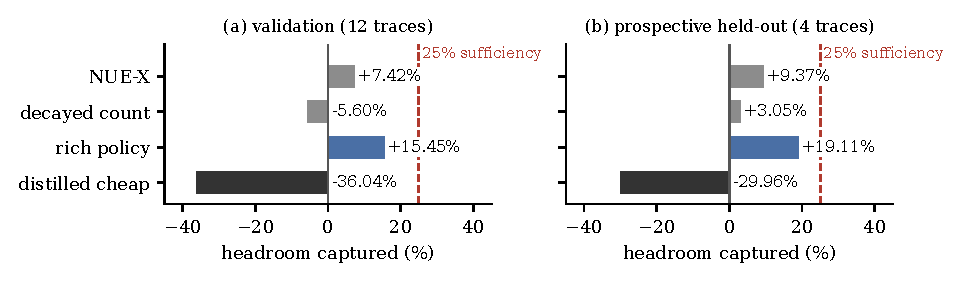
\includegraphics[width=\linewidth]{figures/fig2_capture.pdf}
\caption{Headroom captured (Eq.~\eqref{eq:capture}) by each causal policy on (a) the validation cohort and (b) the prospective held-out evaluation. The dashed line is the frozen sufficiency level of $25\%$; the clairvoyant reference itself ($100\%$) is off scale. Negative bars are policies that incur more miss bytes than the baseline.}
\label{fig:capture}
\end{figure}

\begin{table}[t]
\centering
\caption{Headroom capture (Eq.~\eqref{eq:capture}) of each causal policy against the clairvoyant reference, on the validation cohort (12 traces) and on the prospective held-out evaluation (4 traces). A negative value means the policy incurs more miss bytes than the baseline. The last column states whether the policy reaches the frozen sufficiency level of $25\%$ on both splits.}
\label{tab:results}
\small
\begin{tabular}{llrrc}
\toprule
Policy & Class & Validation & Held-out & $\ge 25\%$ on both \\
\midrule
\textsc{nue-x} & causal, hand-built & $+7.42\%$ & $+9.37\%$ & no \\
decayed count & causal, hand-built & $-5.60\%$ & $+3.05\%$ & no \\
rich policy & causal, learned (GBRT) & $+15.45\%$ & $+19.11\%$ & no \\
distilled cheap policy & causal, learned (CART, depth 3) & $-36.04\%$ & $-29.96\%$ & no \\
\bottomrule
\end{tabular}
\end{table}


The two hand-built comparators are weak: \nuex{} captures $7.42\%$ (positive on all twelve traces, at most $11.19\%$ on any one) and decayed count captures $-5.60\%$, being worse than the baseline on eight of the twelve traces. The rich policy captures $15.45\%$; it is positive on every validation trace but never exceeds $19.59\%$ on a single trace and never reaches $25\%$. The distilled cheap policy captures $-36.04\%$: it incurs 546{,}404{,}401{,}152 more miss bytes than the baseline, $15.00\%$ above it, and is worse than the baseline on all twelve traces, between $-16.13\%$ and $-48.03\%$ (Table~\ref{tab:valtr}). Neither the cheap policy nor the rich policy satisfies its validation requirement.

\paragraph{Sensitivity.} Excluding the validation trace that coincides with the canonical stream of the preceding study changes the pooled captures negligibly: $7.40\%$ for \nuex{}, $-6.14\%$ for decayed count, $15.52\%$ for the rich policy and $-35.42\%$ for the cheap policy. This analysis was non-gating.

%=====================================================================
\section{Prospective Held-Out Evaluation}
\label{sec:evalres}

After the fitted models and the validation scores were hash-locked, the four held-out traces were opened once and all six arms (baseline, reference and four policies) were replayed once on each, 24 executions in total with no recomputation. Pooled decode miss bytes are 1{,}226{,}910{,}965{,}760 for the baseline and 713{,}408{,}901{,}120 for the clairvoyant reference; the recoverable headroom is 513{,}502{,}064{,}640 bytes, $41.85\%$ of the baseline's miss bytes (Table~\ref{tab:miss}).

\begin{table}[t]
\centering
\caption{Pooled decode miss bytes on the four prospective held-out traces at the 1.5~GiB budget, and the change relative to the baseline $A$ in bytes and in percent. The clairvoyant row is the reference used to define recoverable headroom; it is not a causal policy.}
\label{tab:miss}
\small
\begin{tabular}{lrrr}
\toprule
Policy & miss bytes & change vs.\ $A$ (bytes) & change vs.\ $A$ (\%) \\
\midrule
baseline $A$ & 1{,}226{,}910{,}965{,}760 & --- & --- \\
clairvoyant reference & 713{,}408{,}901{,}120 & $-$513{,}502{,}064{,}640 & $-41.85\%$ \\
\textsc{nue-x} & 1{,}178{,}778{,}341{,}376 & $-$48{,}132{,}624{,}384 & $-3.92\%$ \\
decayed count & 1{,}211{,}255{,}119{,}872 & $-$15{,}655{,}845{,}888 & $-1.28\%$ \\
rich policy & 1{,}128{,}796{,}803{,}072 & $-$98{,}114{,}162{,}688 & $-8.00\%$ \\
distilled cheap policy & 1{,}380{,}736{,}696{,}320 & $+$153{,}825{,}730{,}560 & $+12.54\%$ \\
\bottomrule
\end{tabular}
\end{table}


The ordering of the policies is that of validation (Table~\ref{tab:results}, Figure~\ref{fig:capture}(b)). \nuex{} captures $9.37\%$ and decayed count $3.05\%$, saving $3.92\%$ and $1.28\%$ of the baseline's miss bytes. The rich policy captures $19.11\%$, saving 98{,}114{,}162{,}688 bytes ($8.00\%$ of the baseline's miss bytes), $5.89$ percentage points below the sufficiency level; its capture lies between $15.83\%$ and $21.92\%$ on the four workloads. The distilled cheap policy captures $-29.96\%$: it incurs 153{,}825{,}730{,}560 more miss bytes than the baseline ($12.54\%$ above it) and is negative on every workload (Table~\ref{tab:evalwl}). It exceeds the better of the two hand-built comparators on none of the four workloads.

\begin{table}[t]
\centering
\caption{Headroom capture on each held-out evaluation trace (one trace per workload category). The distilled cheap policy is worse than the baseline on every workload.}
\label{tab:evalwl}
\small
\begin{tabular}{lrrrr}
\toprule
Workload & \textsc{nue-x} & decayed count & rich policy & distilled cheap policy \\
\midrule
coding & $+8.86\%$ & $+0.07\%$ & $+15.83\%$ & $-33.08\%$ \\
instruction & $+9.11\%$ & $+3.66\%$ & $+19.00\%$ & $-36.02\%$ \\
reasoning & $+10.24\%$ & $+2.37\%$ & $+19.29\%$ & $-18.89\%$ \\
summarization & $+9.29\%$ & $+5.72\%$ & $+21.92\%$ & $-31.57\%$ \\
\bottomrule
\end{tabular}
\end{table}


As a non-gating description of sampling variability, a block bootstrap over 32 contiguous 64-token decode blocks (2{,}000 resamples, fixed seed) gives 90\% intervals of $[7.71\%, 11.11\%]$ for \nuex{}, $[-1.76\%, 8.06\%]$ for decayed count, $[16.41\%, 21.93\%]$ for the rich policy and $[-36.90\%, -23.45\%]$ for the cheap policy. The interval of the rich policy lies entirely below $25\%$ and that of the cheap policy entirely below $0$. With four held-out traces these intervals describe resampling within the evaluated streams, not variability across prompts or workloads.

%=====================================================================
\section{Causal-State Sufficiency Analysis}
\label{sec:analysis}

\begin{proposition}[Insufficiency under the frozen rule]
\label{prop:main}
Under the frozen decision rule, none of the tested causal policies captures at least $25\%$ of the clairvoyant headroom on both the validation cohort and the prospective held-out evaluation. Consequently the cheap policy fails Rule~A, the rich policy fails the information gate, and the study is classified as causal-state insufficient.
\end{proposition}
\begin{proof}
By Table~\ref{tab:results} the largest validation capture of any policy is $15.45\%$ (rich policy) and the largest held-out capture is $19.11\%$ (rich policy), both below $25\%$. The cheap policy's captures, $-36.04\%$ and $-29.96\%$, fail Rule~A, and the rich policy's captures fail the information gate. The sixth row of Table~\ref{tab:classes} applies: not~A and the information gate fails. Rules~B and~C do not change this outcome, and $24.999\%$ would still have failed.
\end{proof}
The proposition is a statement about the tested policies, the frozen feature vocabulary and the frozen threshold in one regime. It is not a theorem about causal eviction in general.

\subsection{Remaining Gap to the Clairvoyant Reference}
\label{sec:gap}
The best tested causal policy leaves most of the headroom unrecovered. The rich policy recovers $8.00\%$ of the baseline's miss bytes on the held-out traces where the reference recovers $41.85\%$; it leaves $80.89\%$ of the held-out headroom (415{,}387{,}901{,}952 bytes) and $84.55\%$ of the validation headroom unrecovered. It is $9.55$ and $5.89$ percentage points short of the sufficiency level on validation and held-out data.

\subsection{Rich State Versus Simple Causal State}
\label{sec:richsimple}
Richer causal state helps materially. The rich policy captures about twice as much as the best hand-built comparator ($2.04$ times on held-out data and $2.08$ times on validation), and exceeds \nuex{} on all sixteen traces. Decayed count, the simplest recency--frequency rule, does not solve the problem: it is negative on validation and barely positive on held-out data. The improvement from richer state is therefore real but insufficient by the preregistered standard.

\subsection{Distillation Collapse}
\label{sec:distill}
Compressing the rich policy into the constrained rule destroys the value rather than merely reducing it: the cheap policy is $51.50$ percentage points below the rich policy on validation and $49.06$ percentage points below it on held-out data, and below the baseline. A non-gating diagnostic on the training traces measures how often a policy's victim coincides with the teacher's victim (the candidate with the farthest next use): $12.46\%$ of 6{,}951 sampled decisions when the cache state is the baseline's trajectory on which the labels were generated, and $3.76\%$ of 7{,}846 sampled decisions when the cheap policy runs on its own cache states. This is consistent with distribution shift between the labelling trajectory and the states induced by the learned policy, but the study did not isolate the cause of the collapse. Plausible contributors that it did not separate are the coarse ranking (an eight-leaf tree assigns only eight distinct ranks, with recency breaking ties), the restriction to four features, and the mismatch of training and deployment states.

\subsection{Cross-Workload Consistency}
\label{sec:consistency}
The result is not driven by a single workload. The cheap policy is negative on all sixteen traces (Tables~\ref{tab:evalwl} and~\ref{tab:valtr}), \nuex{} is positive on all sixteen but never above $11.19\%$, and the rich policy is positive on all sixteen but never above $21.92\%$ on any single trace (Figure~\ref{fig:pertrace}). No policy reaches $25\%$ on any individual trace.

\begin{figure}[t]
\centering
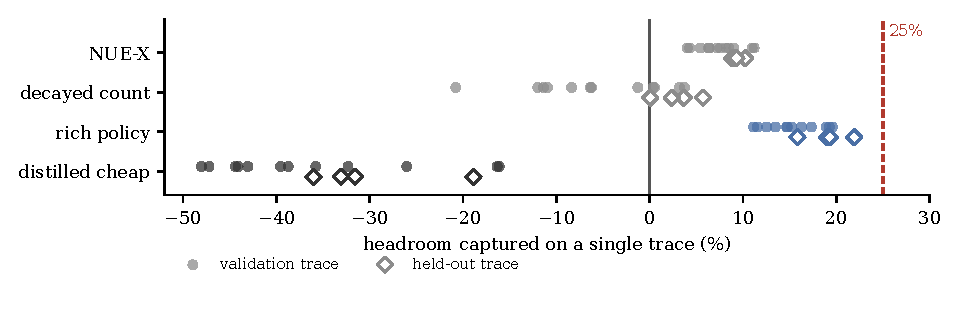
\includegraphics[width=\linewidth]{figures/fig3_pertrace.pdf}
\caption{Headroom captured on every individual trace: circles are the twelve validation traces and diamonds the four held-out traces. The dashed line is the sufficiency level of $25\%$. No policy reaches it on any trace, and the distilled cheap policy is below zero on all of them.}
\label{fig:pertrace}
\end{figure}

\subsection{Why Runtime Overhead Is Not the Whole Explanation}
\label{sec:overhead}
Every number in this study is a miss-byte count from exact offline replay, with no charge for the time taken to compute an eviction decision, and the rich policy's inference cost is ignored by construction. The shortfall is therefore a property of policy quality: with free computation, the best tested causal policy recovers less than a fifth of the held-out headroom, and the policy cheap enough to deploy is worse than the baseline. This complements, and does not replace, the cost attribution of the preceding study: overhead can reduce the value of a retention policy further, but it is not what limits the tested policies here.

%=====================================================================
\section{Relationship to Earlier Argine Results}
\label{sec:related}

\subsection{Predictive Structure and Headroom}
The first study~\cite{argine2paper} established that routing has measurable predictive structure, that clairvoyant headroom exists, and that a predictor-driven policy lowers miss bytes in offline replay. The present result does not contradict those findings: headroom does exist here too ($41.63\%$ and $41.85\%$ of the baseline's miss bytes), and the causal policies do capture some of it. What it adds is a measurement of \emph{how much} of the headroom causal policies can recover.

\subsection{Runtime Falsification of Prediction-Led Retention}
The second study~\cite{argine3paper} showed that predictive structure does not automatically become runtime retention value: in its regime the corrected predictive policy lost $15.83$~ms/token (95\% CI $[10.46, 21.19]$), and the best tested causal next-use policy captured $8.79\%$ of the headroom on its canonical stream. The \nuex{} comparator here is that policy, re-scored on new traces under a new replay, and its capture of $7.42\%$ (validation) and $9.37\%$ (held-out) is of the same order as the earlier figure. The earlier study could not say whether a better causal policy would change the conclusion; the present one gives a prospective answer for a richer causal state.

\subsection{What the Causal-State Experiment Eliminates}
Taken together, the three studies separate three questions: whether predictive \emph{signal} exists (it does), whether the signal can be turned into a policy of good \emph{quality} (not to the preregistered level here), and whether a policy yields \emph{runtime value} once its cost is charged (not in the tested regime). The present result removes a specific explanation of the earlier negative result, namely that a richer causal decision rule would recover enough of the oracle opportunity to rescue prediction-led retention in this regime. It does not remove other explanations, and it does not address mechanisms outside eviction quality.

%=====================================================================
\section{Limitations and Claim Boundary}
\label{sec:claims}

\subsection{What Is Established, What Is Less Plausible, What Is Unknown, and What Is Not Shown}
\paragraph{Established.} In the frozen regime, none of the tested causal policies (two hand-built, one rich learned, one distilled cheap) recovers $25\%$ of the clairvoyant miss-byte headroom on both validation and prospective held-out data. The rich learned policy is better than the hand-built ones by about a factor of two, below the threshold. The distilled cheap policy is worse than the baseline on all sixteen traces. The study's classification follows mechanically from these values.
\paragraph{Made less plausible.} That this causal feature vocabulary, with a boosted-tree learner, is enough to recover most of the oracle headroom; that the tested distillation route yields a deployable policy that preserves the rich policy's value; and that predictor runtime overhead alone explains the earlier negative runtime result.
\paragraph{Unknown.} Whether other causal state (for example longer histories or router-side features), other learners, iterative imitation under the learner's own states, or other training signals would recover more; how much of the clairvoyant headroom is causally attainable at all; and how the policies behave on other models, hardware, budgets and workloads.
\paragraph{Not shown.} The study does not show that every causal or every learned eviction policy is impossible, that no richer representation could work, that no future-aware mechanism could work, that Belady headroom is practically attainable, that expert retention is fundamentally impossible, that other systems mechanisms cannot yield speedups, or that expert-cache strategies are futile.

\subsection{Limitations}
\begin{itemize}
\item \textbf{Regime.} One model (Qwen3-30B-A3B-Q4\_K\_M), one runtime lineage, one expert budget (1.5~GiB) for scoring, offline replay with demand admission and event-atomic multi-key events; traces captured at a different budget (4~GiB) and replayed, which is valid because routing does not depend on the budget.
\item \textbf{Workloads.} Four workload categories, four training traces, twelve validation traces and four held-out traces (one per category). Confidence intervals describe resampling within streams and not variability across prompts.
\item \textbf{Representation and model families.} Sixteen frozen, past-only integer features; one gradient-boosted tree configuration and one depth-3 tree. Different features, learners, hyperparameters or labels were deliberately not explored after the freeze, so the negative result concerns this family and not a search over families.
\item \textbf{Cheap-policy constraints.} Depth at most three, at most four features, integer arithmetic and a single labelling trajectory. The distillation procedure did not iterate between learner and teacher states.
\item \textbf{Policy level versus runtime throughput.} All results are miss bytes in exact replay. No wall-clock throughput was measured and no model was run.
\item \textbf{The reference is not a target.} The clairvoyant reference needs future knowledge and is not proven optimal for multi-key, two-size events; the recoverable headroom is a comparator-relative margin, and a capture of $100\%$ is not a realistic goal.
\item \textbf{Generalization.} Conclusions do not extend to other models, hardware, runtimes or memory budgets without new evidence.
\end{itemize}
These limitations define the scope of the result; they do not qualify the measured values within that scope.

%=====================================================================
\section{Implications for Future Research}
\label{sec:future}

The result bears on prediction-led and causal-eviction retention in the tested regime. It motivates, without establishing anything about, mechanisms that do not depend on eviction quality alone, for example hiding transfer latency by overlapping transfer with computation, scheduling expert transfers, placement, prefetch orchestration, reducing the stall time exposed to the user, reducing the bytes moved per unavoidable miss, and heterogeneous precision or storage strategies. None of these has been tested in this series, and none is specified or begun here.

%=====================================================================
\section{Conclusion}
\label{sec:conclusion}

A substantial clairvoyant expert-retention opportunity exists in the frozen regime, but the tested causal policies recover too little of it. Hand-built causal comparators capture at most $7.42\%$ and $9.37\%$ of the headroom on validation and held-out data, a rich learned policy captures $15.45\%$ and $19.11\%$, and a cheap deployable tree distilled from it captures $-36.04\%$ and $-29.96\%$, against a preregistered sufficiency level of $25\%$ on both. Because computation is not charged, the shortfall is one of causal state and model class, and not merely of predictor overhead. Within the frozen feature vocabulary, model families and regime, causal-state insufficiency is therefore an obstacle to prediction-led expert retention. The result is bounded to that family and regime, and it leaves open every mechanism outside it.

\bibliographystyle{plain}
\bibliography{research4}

\appendix
\section{Provenance}
\label{app:prov}
This appendix is the only place where the repository's internal numbering is used. In that numbering the first study is Research~2, the second is Research~3 and the present study is Research~4; the reader-facing stage names used in the text map to repository identifiers as listed below. Every number in this paper is regenerated from the frozen artifacts by \code{paper/research4/scripts}, and \code{SOURCE\_MAP.md} maps each claim to its artifact and field. The closure record~\cite{argine4evidence} binds the artifacts below.

\begin{table}[h]
\centering
\caption{Present study: reader-facing stage, repository identifier, commit and contract digest (SHA-256).}
\label{tab:prov}
\small
\begin{tabularx}{\linewidth}{>{\raggedright\arraybackslash}p{0.22\linewidth}>{\raggedright\arraybackslash}p{0.2\linewidth}>{\raggedright\arraybackslash}X}
\toprule
Reader-facing name & Repository ID & Commit; contract digest; freeze (SHA-256) \\
\midrule
Causal-State Protocol Freeze & R4-00 & commit \hsh{35410947d51895326aa7e6c39a09825e2ffb4c0c}; digest \hsh{fa0ff8d4c93b463a99bdba4a65625251fa00c8102f5b2d788f8f22e73a20d64e}; freeze \hsh{41e9aa82fcf59155b6c98504ff08bee6ca2feb74027675e3fbce10778ca318be} \\
Model Training and Validation & R4-01 & implementation commit \hsh{db84d702989a3334578b00c1922063056118cd94}; locked commit \hsh{e46df73992ec64e829eddce63e3d50e65bdbd434}; digest \hsh{8d89ecd8198db93000456cde58f995e4fa23124d554402b61170a776d9a0e74f}; freeze \hsh{dbea96e96a386286e49b93e733fb1ed68b5fe22771d9b4d9cf7d8cf55f1756d5} \\
Prospective Evaluation and Classification & R4-02 & opening commit \hsh{30e37fdb0063ed96fa9b9a2d9350bf71a538830e}; digest \hsh{1b690816e6625333fbcac5bf188934ef2f51dbf8ab82ecd1ae7b59c3f02065e0}; freeze \hsh{fc411ef578decf6f7f380832885651f278d8696d9f46d60d2c9d10dce0cb1fdd} \\
\bottomrule
\end{tabularx}
\end{table}

\paragraph{Frozen labels.} The final classification label is \code{R4\_CFDC\_CAUSAL\_STATE\_INSUFFICIENT} and the state label is \code{R4\_CFDC\_CLOSED}; the preceding study's final label is \code{R3\_CLOSED\_NEGATIVE\_PREDICTIVE\_RETENTION\_NOT\_VIABLE\_IN\_TESTED\_REGIME} (closure freeze \hsh{760a22d69abdd207c7ecd4b4f1012b85711b20aa3cb623cddb55d0c8802a5717}). The classification label denotes the sixth row of Table~\ref{tab:classes}.

\paragraph{Execution notes.} The held-out evaluation comprised 24 (trace, policy) executions, none recomputed. The rich-policy replays ran in resumable chunks; two resume invocations were accidentally started concurrently, both resuming from the same atomically written checkpoints of a deterministic computation, so no completed result was duplicated or altered (the recorded per-unit chunk counts and durations may include redundant resumed work). A report-only replicate on a second development seed and a held-out teacher-agreement diagnostic were specified as non-gating and were not computed.

\paragraph{Raw traces.} The routing traces are not part of the repository; each is identified by a SHA-256 recorded in the frozen records, and the replays verified every hash before reading. The four held-out traces are:
\begin{itemize}[itemsep=0pt]
\item coding: \hsh{46104e88a19136153d3223862cd392181d80cc6bfc07e063f009cb7347a392d3}
\item reasoning: \hsh{9adc1ce8801b766fffe64fc54ffc80c7b7bf6dc16b7fe46bcc5c0b3c9a87c0ae}
\item summarization: \hsh{e33fa1e2951498c8e03b6c7fb9e967040e6eae7c8a638e0e2b4ca083e5c8ae33}
\item instruction: \hsh{6a51113fc830b63fc1b8a60c394e16f84df2ff04fb2a566dd1653a96f202dd50}
\end{itemize}

\paragraph{Reproduction.} From the repository root: \code{python}~\code{paper/research4/scripts/build\_assets.py} regenerates tables, figure data and figures from the frozen artifacts; \code{python}~\code{paper/research4/scripts/verify\_paper.py} recomputes every numerical claim, checks the source map, the generated assets, the provenance values and the PDF hash, and fails on any drift; the scientific verifiers of the three stages are run through \code{shared/tooling/run\_frozen\_verifier.py}.

\section{Feature Vocabulary}
\label{app:feat}
The sixteen frozen features of a candidate expert $k$ at an eviction decision, all integer-valued and computed from past requests and the current cache state only: events since last reference; 0.99-decayed request count (fixed point); events since admission; hits since admission; number of previous admissions (reloads); previous reuse interval; mean reuse interval; membership in the layer's previous event; cache occupancy; number of pending misses of the current event; recency rank; frequency rank; expert size in bytes; layer; expert identifier; and layer-cycle offset. Sentinel values denote missing history. The frozen contract forbids any next-use index, any future request, any teacher quantity and any predictor output as an input.

\section{Fitted Cheap Rule}
\label{app:rule}
Among the candidates, evict the one with the highest leaf rank (ties: older last reference, then lower layer, then lower expert). Leaf values are the mean target $y$ of Eq.~\eqref{eq:target} on the training rows of the leaf.
\begin{table}[h]
\centering
\caption{The fitted depth-3 tree (eight leaves, four features). MRI: mean reuse interval; LCO: layer-cycle offset; PM: pending misses of the current event; RC: reload count.}
\label{tab:rule}
\small
\begin{tabular}{lrrr}
\toprule
Condition & rank & mean $y$ & training rows \\
\midrule
MRI $\le 3$, LCO $\le 20$ & 0 & 5.545 & 501{,}678 \\
MRI $\le 3$, LCO $> 20$ & 1 & 6.753 & 822{,}162 \\
$3 <$ MRI $\le 13$, PM $\le 8$ & 2 & 7.474 & 1{,}863{,}612 \\
$3 <$ MRI $\le 13$, PM $> 8$ & 5 & 11.178 & 51{,}438 \\
$13 <$ MRI $\le 33$, PM $\le 8$ & 3 & 8.880 & 330{,}698 \\
$13 <$ MRI $\le 33$, PM $> 8$ & 7 & 11.933 & 16{,}437 \\
MRI $> 33$, RC $= 0$ & 4 & 9.861 & 128{,}509 \\
MRI $> 33$, RC $> 0$ & 6 & 11.900 & 151{,}460 \\
\bottomrule
\end{tabular}
\end{table}

\clearpage
\section{Validation Traces}
\label{app:val}
\begin{table}[H]
\centering
\caption{Headroom capture on each validation trace (three versions of each workload category). No policy reaches $25\%$ on any individual trace; the distilled cheap policy is negative on all twelve.}
\label{tab:valtr}
\small
\begin{tabular}{lrrrr}
\toprule
Trace & \textsc{nue-x} & decayed count & rich policy & distilled cheap policy \\
\midrule
coding v1 & $+7.55\%$ & $+0.51\%$ & $+14.69\%$ & $-43.05\%$ \\
coding v2 & $+6.40\%$ & $-11.98\%$ & $+11.15\%$ & $-26.04\%$ \\
coding v3 & $+11.19\%$ & $-20.78\%$ & $+12.54\%$ & $-38.72\%$ \\
instruction v1 & $+6.33\%$ & $-11.38\%$ & $+11.55\%$ & $-44.39\%$ \\
instruction v2 & $+10.98\%$ & $+0.38\%$ & $+19.59\%$ & $-32.32\%$ \\
instruction v3 & $+8.18\%$ & $+3.18\%$ & $+18.89\%$ & $-35.78\%$ \\
reasoning v1 & $+9.02\%$ & $-6.25\%$ & $+14.77\%$ & $-16.34\%$ \\
reasoning v2 & $+8.49\%$ & $-10.96\%$ & $+16.24\%$ & $-16.13\%$ \\
reasoning v3 & $+5.42\%$ & $-6.35\%$ & $+15.20\%$ & $-48.03\%$ \\
summarization v1 & $+4.29\%$ & $-8.36\%$ & $+13.46\%$ & $-47.21\%$ \\
summarization v2 & $+4.04\%$ & $-1.26\%$ & $+17.34\%$ & $-44.11\%$ \\
summarization v3 & $+7.23\%$ & $+3.72\%$ & $+19.26\%$ & $-39.55\%$ \\
\bottomrule
\end{tabular}
\end{table}


\end{document}
